\section{当前基准的实证诊断}

\begin{figure}[t]
    \centering
    \resizebox{\textwidth}{!}{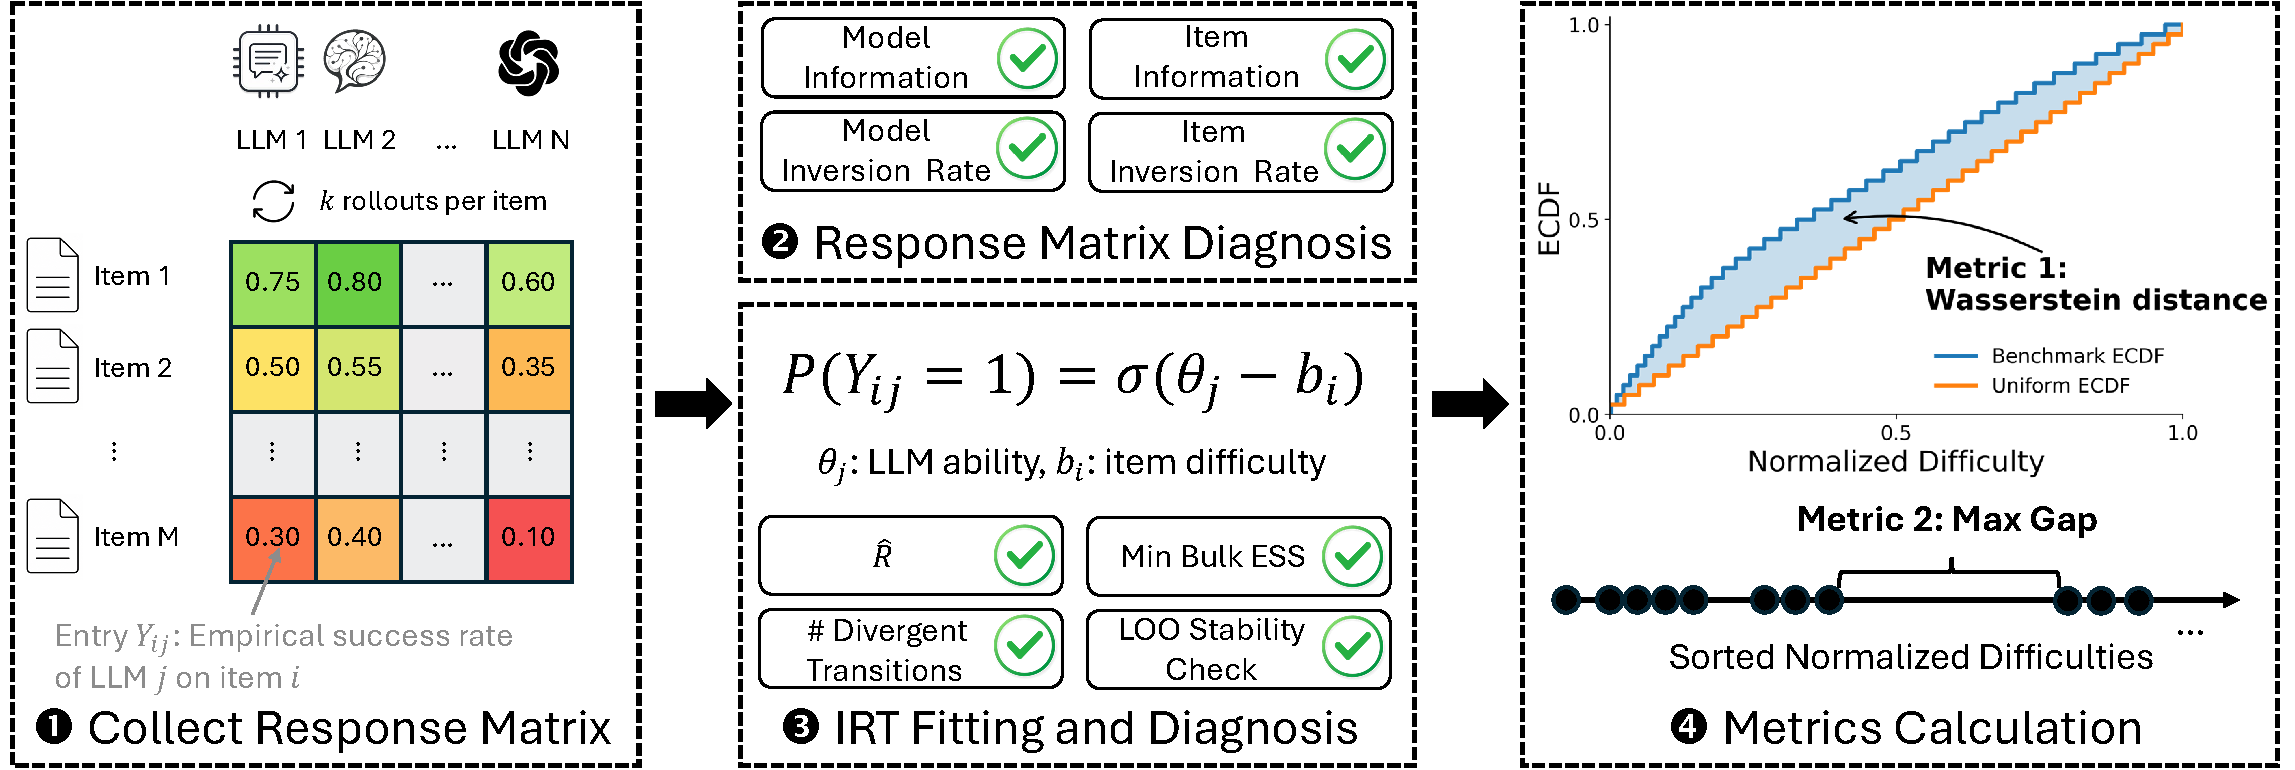
\includegraphics{Fig/pipeline.pdf}}
      \vspace{-4mm}
    \caption{\textbf{基准难度估计与指标计算流程概览。} 我们收集多个 LLM 在基准题目上的经验成功率，诊断响应矩阵，拟合 1PL IRT 模型以估计题目难度，进行拟合后的 IRT 诊断，并在归一化难度分布上计算两个指标。
    % Wasserstein-based distribution mismatch and the maximum adjacent difficulty gap.
    }
    \label{fig:pipeline}
  \vspace{-4mm}
\end{figure}
我们用前文提出的两个指标，分析一组来自不同领域、被广泛使用的基准。图~\ref{fig:pipeline} 给出难度估计与指标计算流程的概览。具体而言，我们考虑涵盖数学、编程、智能体任务、逻辑、科学、指令遵循与医学的 \textbf{25} 个常用基准。这些基准的详细信息见附录~\ref{sec:app_benchmark_details}。

\subsection{难度估计与指标计算}

\paragraph{方法：项目反应理论。}
为估计基准题目难度，人们可能会直接使用每道题在各模型上的平均失败率~\citep{yu2025dapo,sun2026improving,wen2025light}。然而，题目难度本质上相对于模型能力：它不仅应取决于有多少模型答错该题，还应取决于答错或答对该题的模型有多强。
% Average failure rate ignores the abilities of the models behind these successes and failures. 
因此我们使用项目反应理论（IRT）。它是一个成熟的心理测量框架~\citep{lord1952theory, rasch1993probabilistic}，已被广泛用于 LLM 基准分析中的难度估计~\citep{ding2024easy2hard, rodriguez2021evaluation, hofmann2025fluid, kipnis2024metabench, polo2024tinybenchmarks, zhou2026lost}。IRT 将模型解出一道题的概率建模为模型能力与题目难度的函数。在常用的单参数 logistic 模型（1PL）中，每个模型 $j$ 被赋予能力参数 $\theta_j$，每道题 $i$ 被赋予难度参数 $b_i$。模型 $j$ 正确解出题目 $i$ 的概率建模为
\[
\Pr(Y_{ij}=1)=\sigma(\theta_j-b_i),
\]
其中 $\sigma(\cdot)$ 为 logistic 函数。直观上，$b_i$ 越大的题目需要越高的模型能力才能被正确解出，因此估计得到的 $b_i$ 提供了题目难度的自然度量。对选择题基准，上述模型可以自然地用猜测参数加以扩展。

实践中，难度估计首先收集多个模型在基准题目上的表现，形成响应矩阵 $Y \in \mathbb{R}^{n \times m}$，其中 $Y_{ij}$ 表示模型 $j$ 在题目 $i$ 上的经验成功率。随后通过拟合 IRT 模型所诱导的似然，估计潜在能力 $\{\theta_j\}_{j=1}^m$ 与题目难度 $\{b_i\}_{i=1}^n$。
% This is typically done via maximum likelihood or Bayesian estimation methods (e.g., Markov chain Monte Carlo (MCMC) or variational inference). 
为确保难度估计可靠，我们采取若干实际措施，包括\textbf{审慎的模型选择}与\textbf{严格的 IRT 拟合诊断}。

\paragraph{模型选择。}
准确的难度估计需要能力水平多样的模型。为确保充分的能力覆盖，我们有意选择跨越宽能力范围的模型。对非智能体基准，我们依据 Text Arena 的公开排行榜\footnote{\url{https://arena.ai/leaderboard}} 选择 $12$ 个 LLM，参数规模从 $1.7$B 到 $397$B。模型首先按跨多个领域汇总的总体能力排序，再沿该排名划分为若干近似等长的区间。我们通过从每个区间选取一个模型进行分层抽样，并额外纳入排名顶部与底部的若干模型，以更好地覆盖能力谱的两端。每个被选模型在每道基准题上最多进行 $32$ 次 rollout，使用模型推荐的 temperature 与 top-$p$。对智能体基准，任务通常需要较强的专有模型。因此我们依赖 HAL~\cite{hal} 的评测结果，它报告了 $15$--$66$ 个最先进闭源 LLM 在智能体任务基准上的表现。模型的详细信息见附录~\ref{sec:app_model_details}。

\paragraph{IRT 拟合与诊断。}
我们通过 MCMC 进行贝叶斯推断来估计 IRT 参数。为确保难度估计可靠，我们在 IRT 拟合\textit{之前}与\textit{之后}都进行一系列诊断。拟合前，我们用 $4$ 个指标检查响应矩阵的信息量与结构一致性。拟合后，我们用 $3$ 个标准贝叶斯诊断评估收敛性与采样质量，包括 Gelman--Rubin 统计量（$\hat{R}$）、有效样本量（ESS）以及发散转移的次数。所有基准都通过了全部 $7$ 项诊断检查。
对非智能体基准，我们进一步进行留一法（leave-one-out, LOO）稳健性分析。结果表明，我们选择的 $12$ 个模型足以得到稳定的难度估计。为支持后续工作，我们还公开发布了这 $25$ 个基准经过仔细整理的难度估计\footnote{\url{https://github.com/ASTRAL-Group/benchmark-difficulty-measure/tree/main/data/benchmarks}}。详细定义与诊断结果见附录~\ref{sec:app_irt}。我们还在附录~\ref{app:irt_model_comparison} 中提供了与 2PL 及多维 IRT 模型的额外模型比较分析。

% For non-agentic benchmarks, we further conduct a leave-one-out (LOO) robustness analysis. Specifically, we refit IRT after removing each model in turn, and measure the consistency between the resulting item difficulties and the original estimates. Averaged over the $12$ LOO refits within each benchmark, both the Spearman and Pearson correlations are at least $0.97$ for every benchmark, indicating that our choice of $12$ models is sufficient for stable difficulty estimation. To support future work, we will open-source the carefully curated difficulty estimates for the $25$ benchmarks. Detailed definitions and results are provided in App.~\ref{sec:app_irt}.

% For non-agentic benchmarks, we also perform a leave-one-out robustness analysis over the selected model set; averaged over leave-one-out refits and benchmarks, both the Pearson and Spearman correlations with the original difficulty estimates exceed $0.97$, indicating highly stable difficulty estimation (App.~\ref{sec:app_irt}).

\paragraph{所提出指标的计算。}
对每个基准，在估计题目难度后，我们首先将其归一化到 $[0,1]$，并计算其经验累积分布函数（ECDF）。由于一般情况下难度空间上没有额外先验信息，我们通过计算基准经验测度与 $[0,1]$ 上同规模经验\textit{均匀参照}之间的 1-Wasserstein 距离来量化分布失配。在一维情形下，这等价于它们 ECDF 之间的 $L_1$ 距离。我们按式~\eqref{eq:max_gap} 计算最大间隔，并同时报告五个最大相邻间隔之和作为参照指标。两个指标的后验不确定性分析见附录~\ref{app:metric_uncertainty}。

\subsection{结果与分析}

\paragraph{若干基准相对中性均匀目标存在较大偏离。} 表~\ref{tab:main_result} 显示，25 个基准中有 10 个满足 $\mathrm{DDM}\ge 0.10$，表明其经验难度分布平均至少需要搬运整个难度范围的 10\%，才能与同规模均匀参照相匹配。因此这些基准编码了很强的隐含难度加权：其汇总分数对过度代表的难度区域更敏感，对代表不足的区域更不敏感。当非均匀性与预期评测目标一致时，它本身并非问题。然而，若未指定这样的目标，高 DDM 的排行榜结果不应被解读为难度中性的比较。相反，它们反映的是在该基准经验难度加权下的比较，因此使用者应检查这一加权是否与其使用场景相关的难度分布相符。附录~\ref{sec:app_benchmark_cal} 给出一个简单的基准校准算法，用于使基准分布更接近选定的目标。

\paragraph{许多基准存在较大的局部覆盖缺口。}
表~\ref{tab:main_result} 显示，25 个基准中有 8 个满足 $\mathrm{Max\ Gap}\ge 0.10$。因此，一次训练可能在未被覆盖的难度区域取得有意义的局部进展，而汇总基准分数几乎不变。这会导致有用的训练进展被低估，有希望的运行被过早放弃，计算资源被错误分配。此外，问题并不限于单一的最大间隔。我们发现 25 个基准中有 9 个满足 $\mathrm{Top\text{-}5\ Sum}\ge 0.30$。例如，图~\ref{fig:main_result} 显示 AIME24 与 AIME25 的前 5 大间隔之和接近 $0.5$，尽管它们被广泛用于监测 RLVR 训练~\cite{luo2025deepscaler,liu2025prorl,guo2025deepseek,yue2025vapo}，难度轴上仍有大段局部未分辨。

我们指出，尽管 $\mathrm{Max\ Gap}$ 本质上依赖于基准规模，这反映的是真实的覆盖限制，而不仅仅是需要消除的干扰效应：即使小基准预期会有较大间隔，它仍然是一段未被覆盖的难度区间，并且由定理~\ref{thm:max-gap-detection-boundary}，落在该区间内的局部改进在最坏情形下可能不可检测。重要的是，我们发现覆盖缺口并非仅仅是小基准的产物：拥有数百道题的基准，例如 HumanEval 与 BBH-5 objects，也表现出可观的间隔指标。这促使我们将缺口填补作为提高基准局部分辨率的一种实用且必要的途径。

\begin{figure*}[t]
    \centering
    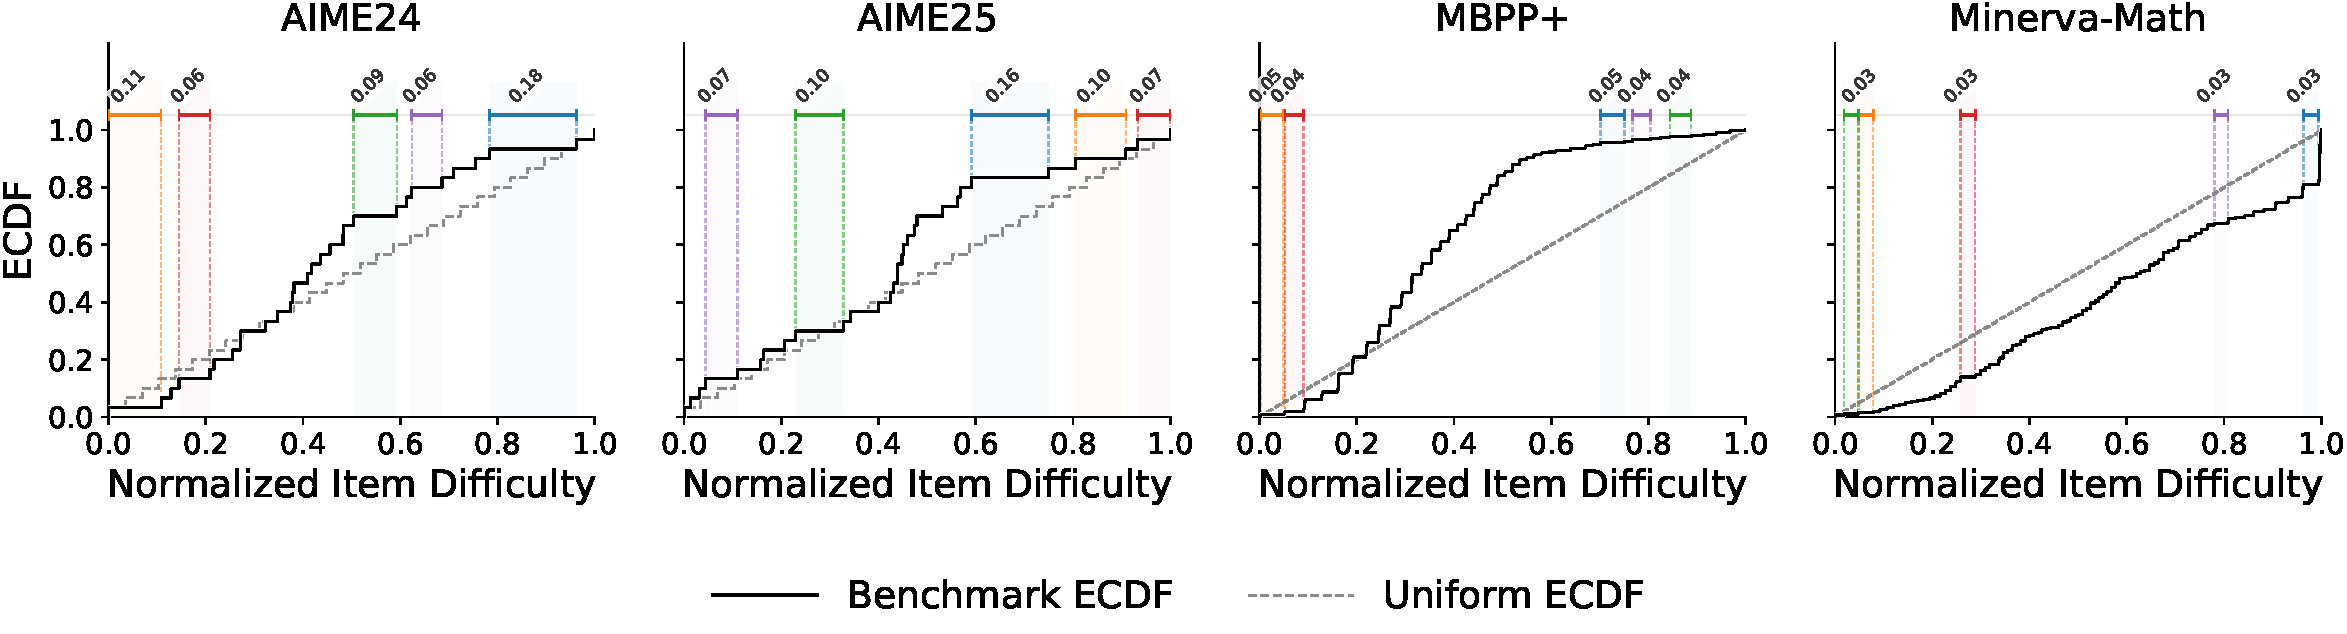
\includegraphics[width=\textwidth]{Fig/main_result.pdf}
  \vspace{-4mm}

    \caption{\textbf{基准难度分布。}
    每个面板展示一个基准归一化题目难度的 ECDF，以及中性均匀参照。彩色阴影区间标出五个最大的相邻难度间隔，标签为相应的间隔大小。更多基准示例见图~\ref{fig:appendix_result}。}
    \label{fig:main_result}
    \vspace{-4mm}
\end{figure*}

\begin{table*}[t]
\centering
\caption{\textbf{各基准上所提出指标的汇总。}
$\mathrm{DDM}$ 表示基准经验难度分布与 $[0,1]$ 上同规模经验均匀分布之间的 1-Wasserstein 距离。$\mathrm{Max\ Gap}$ 是归一化难度相邻点之间的最大间隔，$\mathrm{Top\text{-}5\ Sum}$ 是五个最大此类间隔之和。\# 表示基准题目数。三个指标均越低越好。高亮条目标出各指标相对较大的值：$\mathrm{DDM}\ge 0.10$，$\mathrm{Max\ Gap}$ $\ge 0.10$，或 $\mathrm{Top\text{-}5\ Sum}$ $\ge 0.30$。}
\label{tab:main_result}
\small
\begin{minipage}[t]{0.49\linewidth}
\vspace{0pt}
\centering
\resizebox{\linewidth}{!}{
\begin{tabular}{l r r r r}
\toprule
\textbf{基准} &
\textbf{$\mathrm{DDM}$} & \textbf{$\mathrm{Max\ Gap}$} & \textbf{$\mathrm{Top\text{-}5\ Sum}$} & \textbf{\#} \\
\midrule
MATH-500 & \highddm{0.164} & 0.058 & 0.175 & 500 \\
Minerva-Math & \highddm{0.122} & 0.031 & 0.149 & 272 \\
OlympiadBench & 0.064 & 0.048 & 0.142 & 675 \\
Gaokao2023en & 0.088 & 0.055 & 0.183 & 385 \\
AMC23 & 0.089 & \highddm{0.217} & \highddm{0.539} & 40 \\
AIME24 & 0.077 & \highddm{0.179} & \highddm{0.502} & 30 \\
AIME25 & 0.079 & \highddm{0.158} & \highddm{0.492} & 30 \\
AIME26 & 0.085 & \highddm{0.119} & \highddm{0.507} & 30 \\
MMLU-Pro-Biology & \highddm{0.125} & 0.045 & 0.151 & 717 \\
MMLU-Pro-Chemistry & \highddm{0.114} & 0.072 & 0.192 & 1132 \\
MMLU-Pro-Physics & \highddm{0.121} & 0.035 & 0.157 & 1299 \\
GPQA-Diamond & 0.080 & 0.066 & 0.263 & 198 \\
ScienceQA & \highddm{0.178} & 0.045 & 0.175 & 4241 \\
\bottomrule
\end{tabular}
}
\end{minipage}
\hfill
\begin{minipage}[t]{0.49\linewidth}
\vspace{0pt}
\centering
\resizebox{\linewidth}{!}{
\begin{tabular}{l r r r r}
\toprule
\textbf{基准} &
\textbf{$\mathrm{DDM}$} & \textbf{$\mathrm{Max\ Gap}$} & \textbf{$\mathrm{Top\text{-}5\ Sum}$} & \textbf{\#} \\
\midrule
HumanEval & \highddm{0.148} & \highddm{0.165} & \highddm{0.423} & 164 \\
MBPP+ & \highddm{0.163} & 0.049 & 0.214 & 378 \\
GAIA & 0.084 & 0.051 & 0.218 & 165 \\
CORE-Bench Hard & 0.036 & \highddm{0.113} & \highddm{0.363} & 45 \\
SWE-bench-Mini & 0.053 & \highddm{0.149} & \highddm{0.469} & 50 \\
USACO & 0.080 & 0.082 & \highddm{0.354} & 307 \\
IFEval & \highddm{0.159} & 0.046 & 0.189 & 541 \\
BBH-3 objects & 0.090 & 0.075 & 0.294 & 250 \\
BBH-5 objects & 0.099 & \highddm{0.128} & \highddm{0.332} & 250 \\
BBH-7 objects & 0.077 & 0.059 & 0.279 & 250 \\
ZebraLogic & 0.080 & 0.027 & 0.127 & 1000 \\
MedQA & \highddm{0.157} & 0.042 & 0.178 & 1273 \\
\bottomrule
\end{tabular}
}
\end{minipage}
    \vspace{-4mm}

\end{table*}
